\documentclass[final, usenames, dvipsnames]{beamer}
\usepackage{grffile}

\mode<presentation>{\usetheme{GWU}}
\usepackage[orientation=landscape, scale=1.24,debug]{beamerposter} 
%\beamertemplategridbackground[1in] % grid for aligning stuff
\usepackage{mathtools, amsthm, amssymb, latexsym}
\usepackage[english]{babel} % language hyphenation

\usepackage{graphicx, setspace}
\usepackage{bigstrut, multirow, float}

\usepackage{caption}
\usepackage{subcaption}
\usepackage{xcolor}
\usepackage{multicol}
%\setlength{\abovecaptionskip}{0.1cm}
%\setlength{\belowcaptionskip}{-0.3cm}

\graphicspath{{./figures/}}

\def\newblock{} % Avoid the "\newblock undefined" error. See http://newsgroups.derkeiler.com/Archive/Comp/comp.text.tex/2008-07/msg00381.html"

%-----------------------------------------------------------
\newlength{\colsep}
\newlength{\onecolwidth}
\newlength{\twocolwidth}

\setlength{\paperwidth}{121.92cm} % 48in
\setlength{\paperheight}{91.44cm} % 36in


%\setlength{\onecolwidth}{0.23\textwidth} % Width of one column
%\setlength{\twocolwidth}{0.49\textwidth} % Width of two columns
\setlength{\onecolwidth}{28cm} % Width of one column
\setlength{\twocolwidth}{56cm} % Width of two columns
\newlength{\columnheight}
\setlength{\columnheight}{76.5cm}

\setbeamersize{text margin left=1.5cm,text margin right=0.5cm}

\listfiles

%-----------------------------
% MACROS
%-----------------------------
\def\Emph{\textcolor{RoyalBlue}}
%%%%%%%%%%%%%%%%%%%%%%%%%%%%%%%%%%%%%%%%%%%%%%%%%%%%%%%%%%%%%%%%%%%%%%%%%%%%%%%%%%%%%%
%	TITLE
%%%%%%%%%%%%%%%%%%%%%%%%%%%%%%%%%%%%%%%%%%%%%%%%%%%%%%%%%%%%%%%%%%%%%%%%%%%%%%%%%%%%%%%
\title{\Large Optimal Low Thrust Transfers in the Circular Restricted Three Body Problem}
\author{\Large \textcolor{white}{Shankar Kulumani}}
\institute{\large Flight Dynamics and Controls Laboratory (Dr. Taeyoung Lee)\\Department of Mechanical and Aerospace Engineering, School of Engineering and Applied Science}

%----------------------------------------------------------------------------------------

\begin{document}
\begin{frame}[t] % enclose entire poster in a frame
\begin{columns}[T,onlytextwidth] % start of all columns in poster

%-----------------------------------------------------------------------------------------
% FIRST (LEFT) COLUMN
%---------------------------------------------------------------------------------------
\begin{column}{\onecolwidth} % first column start

\begin{block}{I. Background and Motivation} % Background block
	\begin{itemize}
		\item Spacecraft serve a critical role in enabling and understanding modern life 
			\begin{itemize}
				\item The Global Positioning System (GPS) is vital to navigation, commerce, and emergency services
				\item Scientific instruments such as the Hubble Space Telescope, Voyager missions, and the recent Rosetta mission have provided great insight into our solar system
			\end{itemize}
		\item Designing spacecraft trajectories is a classic and ongoing topic of research
			\begin{itemize}
				\item Predicting the motion of celesial bodies has motivated the likes of Newton, Euler, and Lagrange
				\item The launch of Sputnik in 1957 shifted the focus to the motion of man-made objects
				\item Incorporating additional perturbing forces increases the model accuracy at the expense of complexity
			\end{itemize}
		\item The addition of propulsion devices enables the spacecraft to depart from the free motion trajectory
			\begin{itemize}
				\item Previous work assume impulsive or instantaneous changes in spacecraft velocity (\( \Delta V \)) to ease complexity
				\item Continuous low thrust propulsion devices, such as electric propulsion, increase analysis complexity but improve capability
				\item \Emph{Electric Propulsion} has higher exhaust speeds and offers higher specific impulse than chemical propulsion methods
				\item Can operate for extended periods which is ideal for deep space missions  
			\end{itemize}
		\item Miniaturization of electric propulsion enables their use on small satellites (\( 1 - 100 \text{ kg} \))
		\item Several recent missions have exploited the system dynamics to enable very low energy orbital transfers
	\end{itemize}
	\begin{figure}
        \hspace*{\fill}%
        \begin{subfigure}[b]{0.2\columnwidth}%
                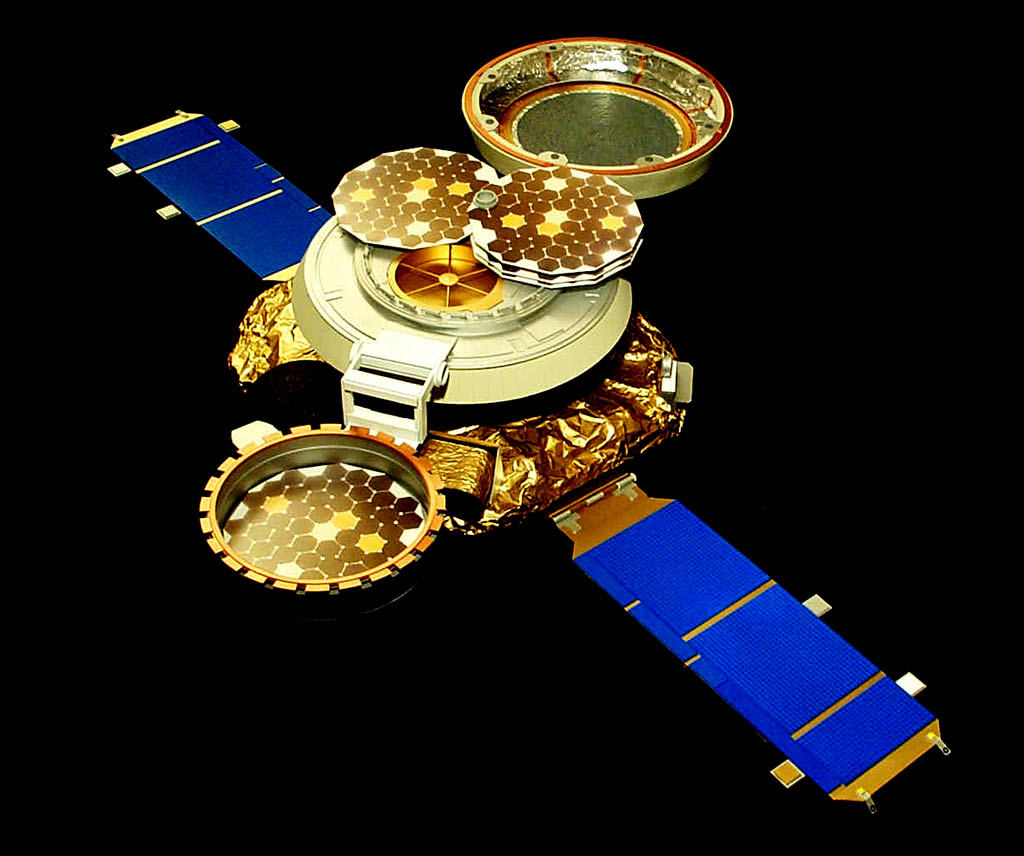
\includegraphics[height=4cm]{genesis_sc}%
                \caption*{Genesis}%
                \label{fig:genesis}%
        \end{subfigure}%
        \hfill%
        \begin{subfigure}[b]{0.2\columnwidth}%
                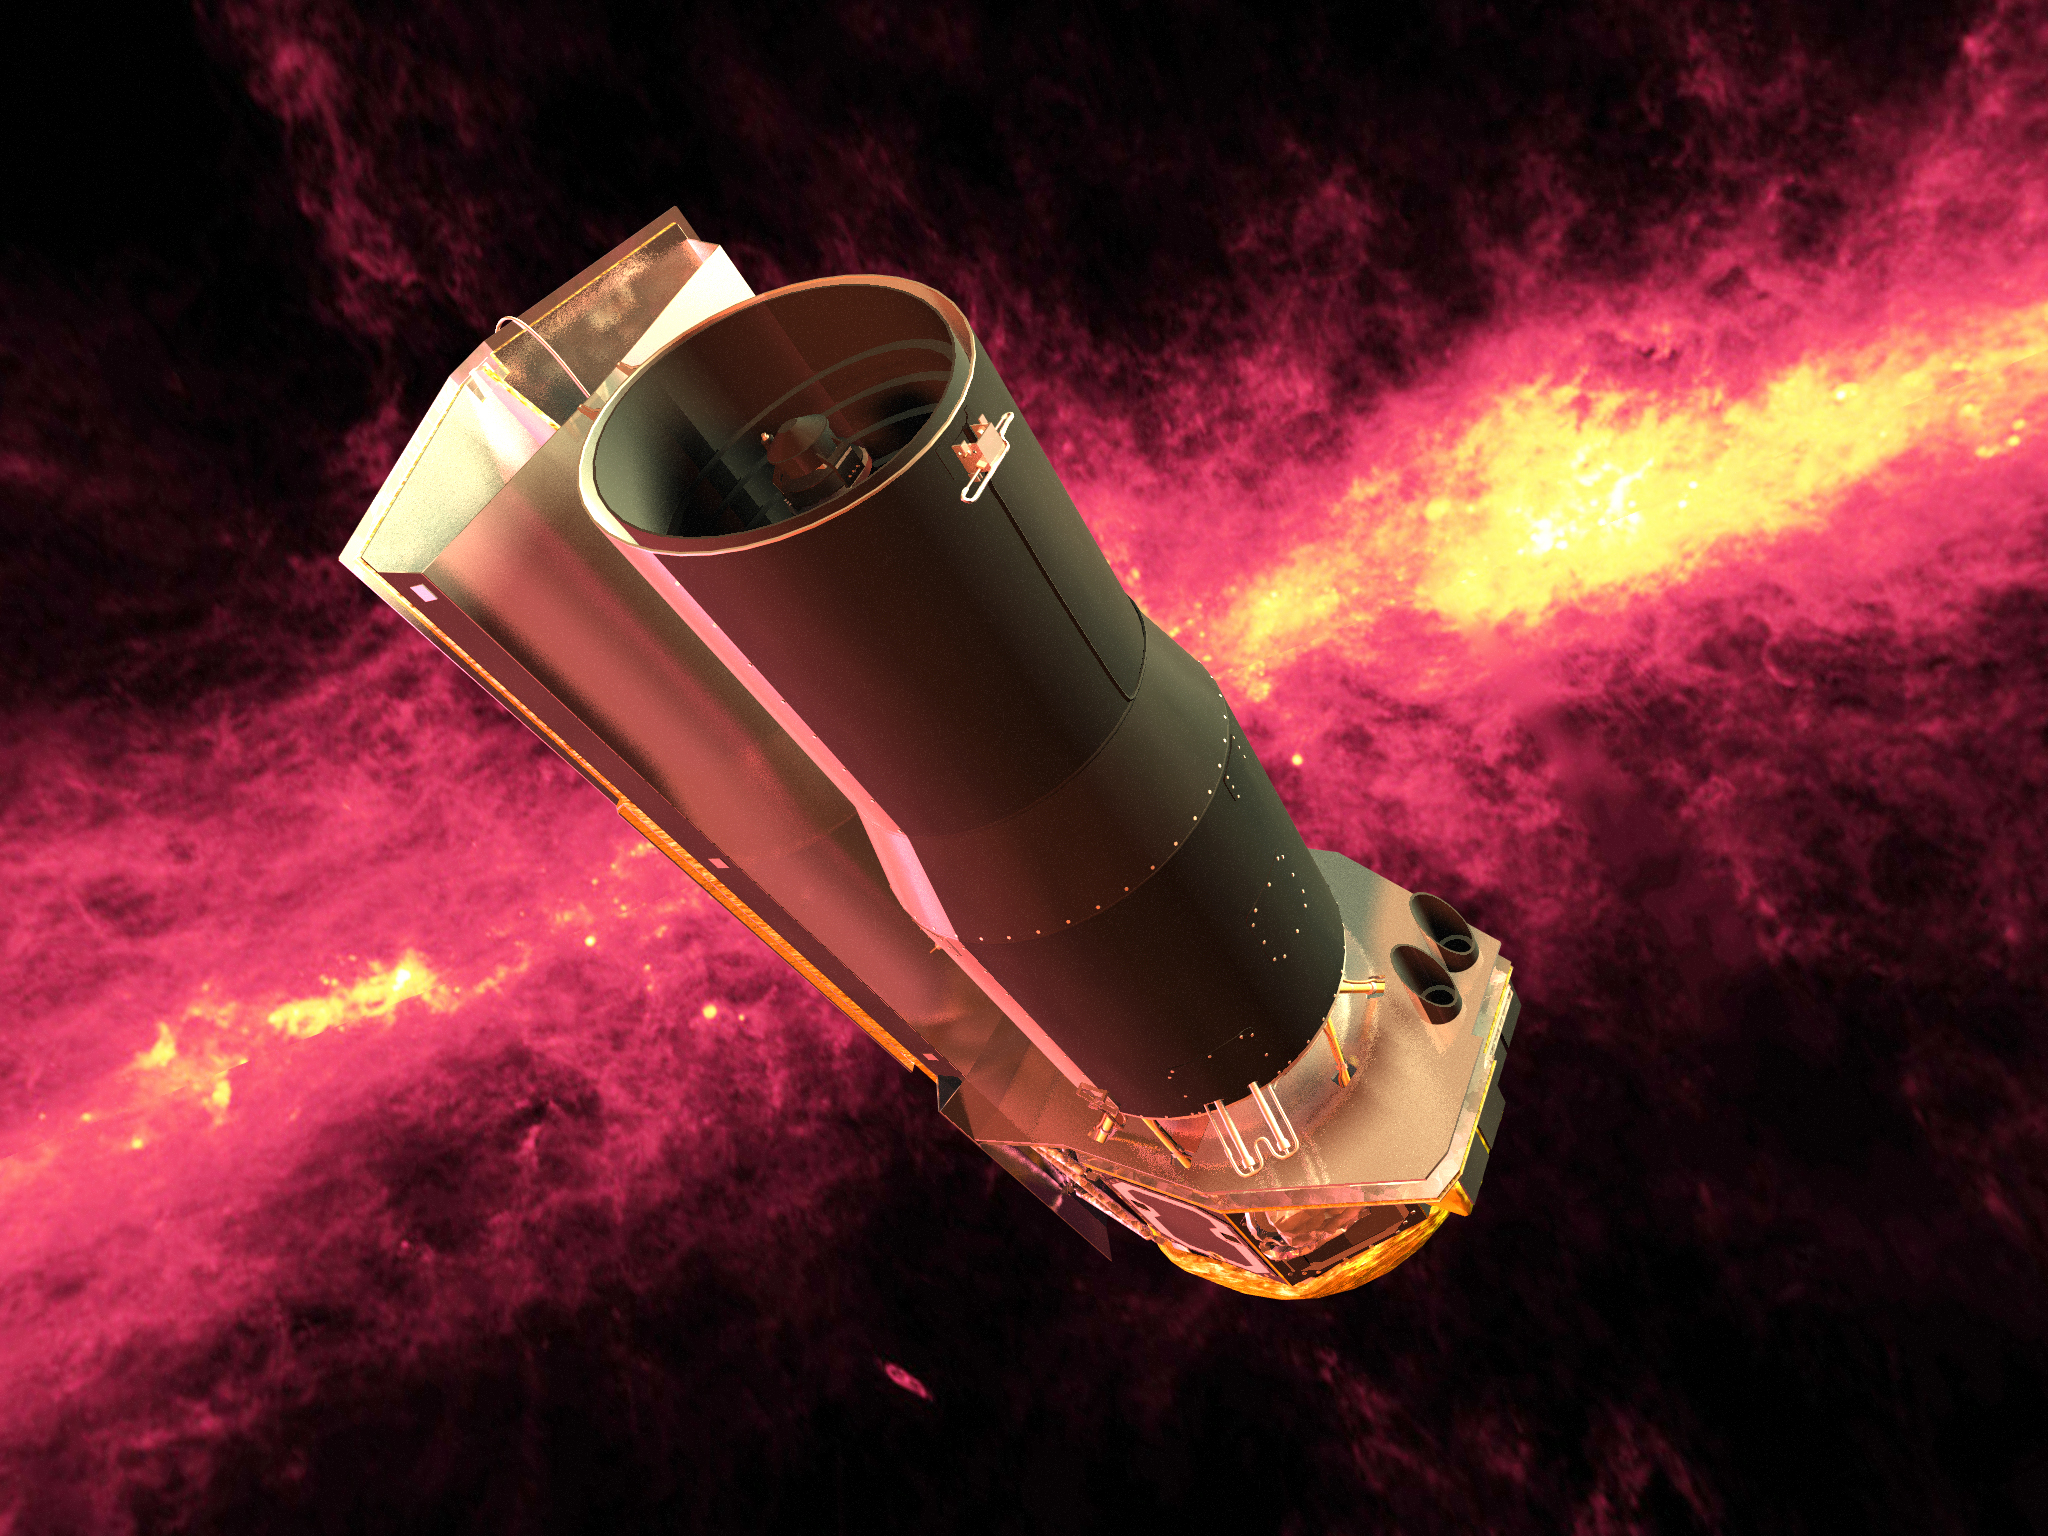
\includegraphics[height=4cm]{spitzer}%
                \caption*{Spitzer}%
                \label{fig:soho}%
        \end{subfigure}%
        \hfill%
		 \begin{subfigure}[b]{0.2\columnwidth}%
            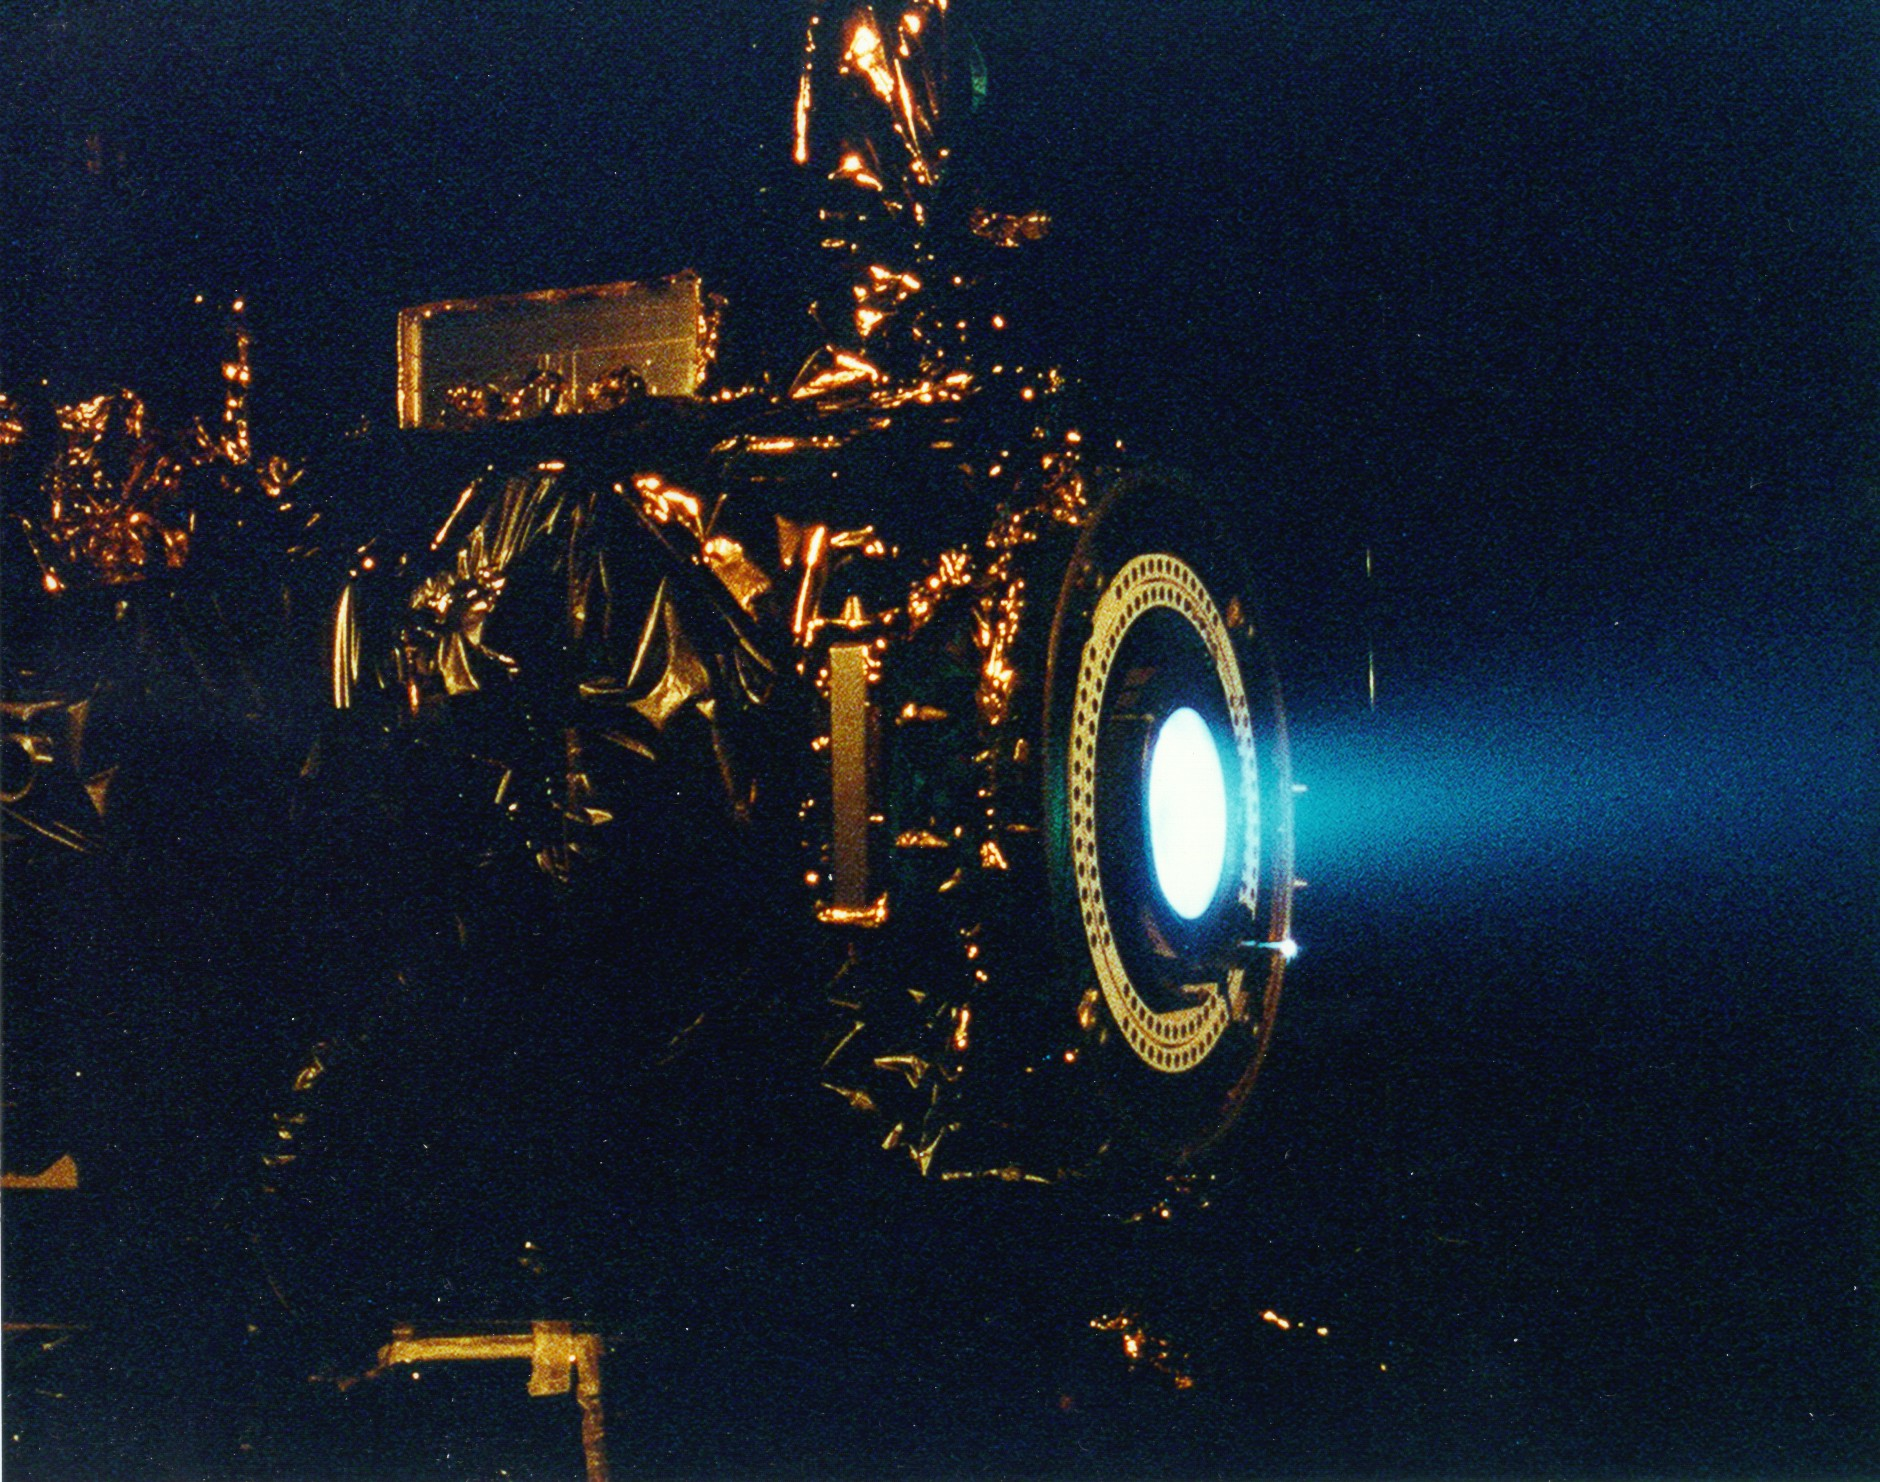
\includegraphics[height=4cm]{nstar_firing}%
            \caption*{Ion Propulsion}%
            \label{fig:isee3}%
        \end{subfigure}%
		\hspace*{\fill}%
		\label{fig:intro}
	\end{figure}
\end{block} % end of background block

\begin{block}{II. Dynamic Model} % dynamics block
	\begin{itemize}
		\item \Emph{Circular Restricted Three Body Problem} describes the motion of a spacecraft under the gravitational force of two massive primaries
			\begin{itemize}
				\item No closed form analytic solutions available
				\item Use of a rotating reference frame allows for additional insight that produces an effective system for trajectory design in a multi-body environment  
			\end{itemize}
			
		\item The \Emph{Jacobi Integral}, is a scalar energy like term that divides realms of possible motion
			 \begin{equation*}
			 	E = \frac{1}{2} \left( \dot{x}^2 + \dot{y}^2 + \dot{z}^2 \right) + \bar{U}(x,y,z)
			 \end{equation*}
	\end{itemize}
	\begin{figure}
		\begin{subfigure}[b]{0.45\columnwidth}
			 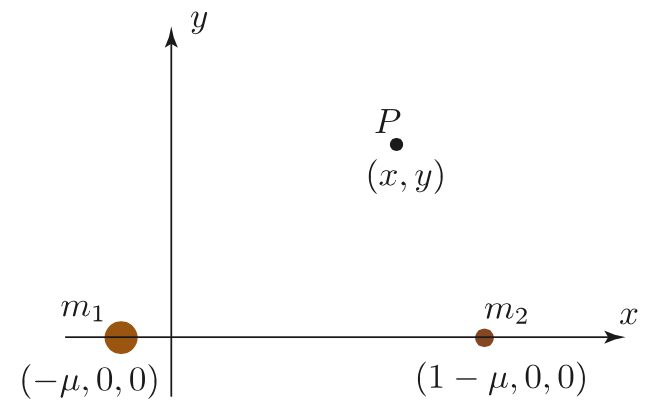
\includegraphics[width = \columnwidth]{rotating_ref_frame}
			\caption*{Rotating Reference Frame\label{fig:rotating_ref_frame}}
		\end{subfigure}%
		\quad%
		\begin{subfigure}[b]{0.45\columnwidth}
			 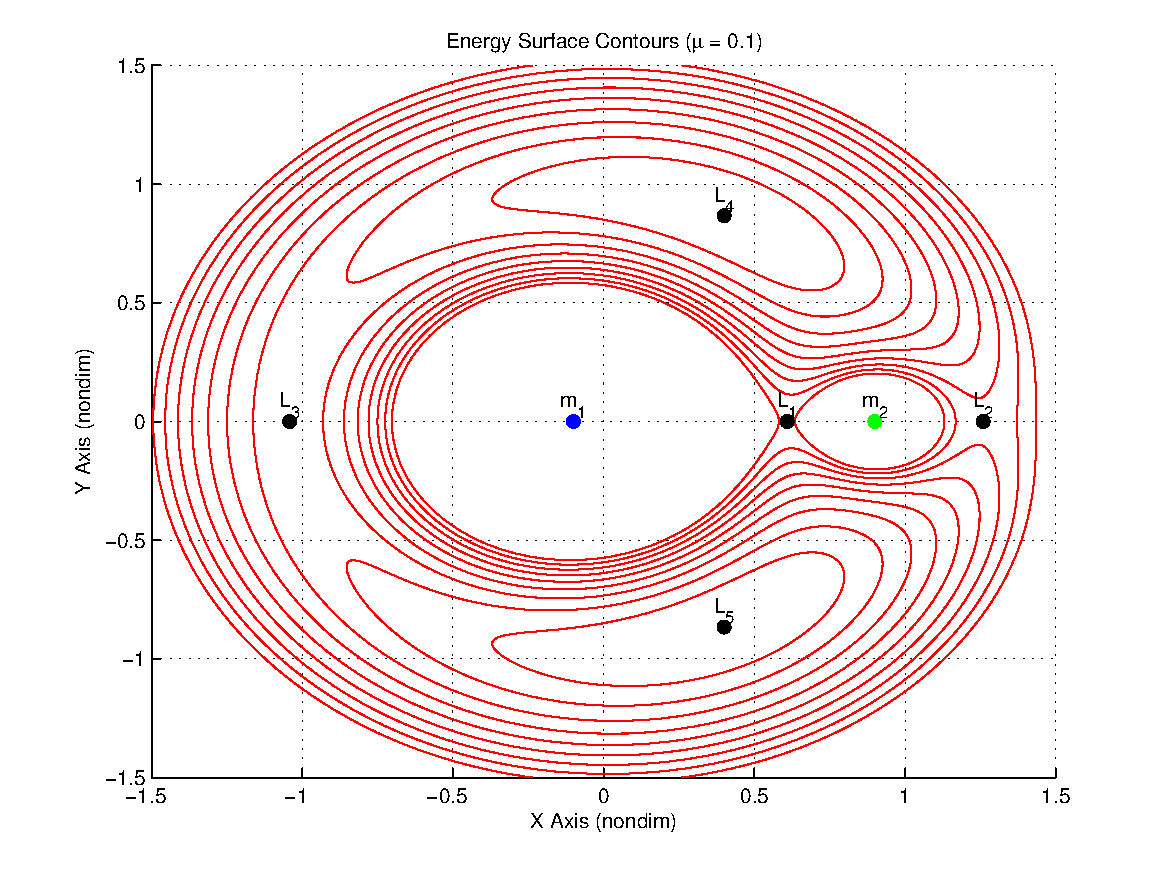
\includegraphics[width = \columnwidth]{energy_contours}
			\caption*{Energy Contours\label{fig:energy_contours}}
		\end{subfigure}
	\end{figure}
\end{block} % end of dynamics block
\end{column}  % first column end

%-----------------------------------------------------------------------------------------
% SECOND (WIDE MIDDLE) COLUMN
%---------------------------------------------------------------------------------------
\begin{column}{\twocolwidth} % second column start

\begin{block}{III. Dynamic Structure} % structure block
	\begin{minipage}{0.5\columnwidth} % left half of this block
	\begin{itemize}
		\item Equilibrium points classified by local stability properties 
			\begin{itemize}
				\item Collinear lagrange points (L1, L2, L3) are dynamically unstable while equilateral (L4, L5) are stable
				\item Numerical technique of \Emph{Differential correction} allows for infinite number of periodic solutions
					\begin{equation*}
						\delta x(t) = \frac{\partial x}{\partial x_0} \delta x_0 = \Phi(t,t_0) \delta x_0
					\end{equation*}
				\item The \Emph{State Transition Matrix} gives the linear relationship between initial and final displacements
					\begin{equation*}
						\dot{\Phi(t,t_0)} = \frac{\partial f(x, u , t)}{\partial x} \Phi(t,t_0)
					\end{equation*}
			\end{itemize}
		\item The \Emph{Monodomy Matrix} of the periodic solutions allows insight into the local stability 
			\begin{equation*}
				M = \Phi(T)
			\end{equation*}
		\item Globalization of the \Emph{Invariant Manifolds} define regions of the state space that asymptotically arrive or depart the periodic orbit
	\end{itemize}
	\end{minipage}% end of left half of block
	\begin{minipage}{0.5\columnwidth}% right half of block
		\begin{figure}
			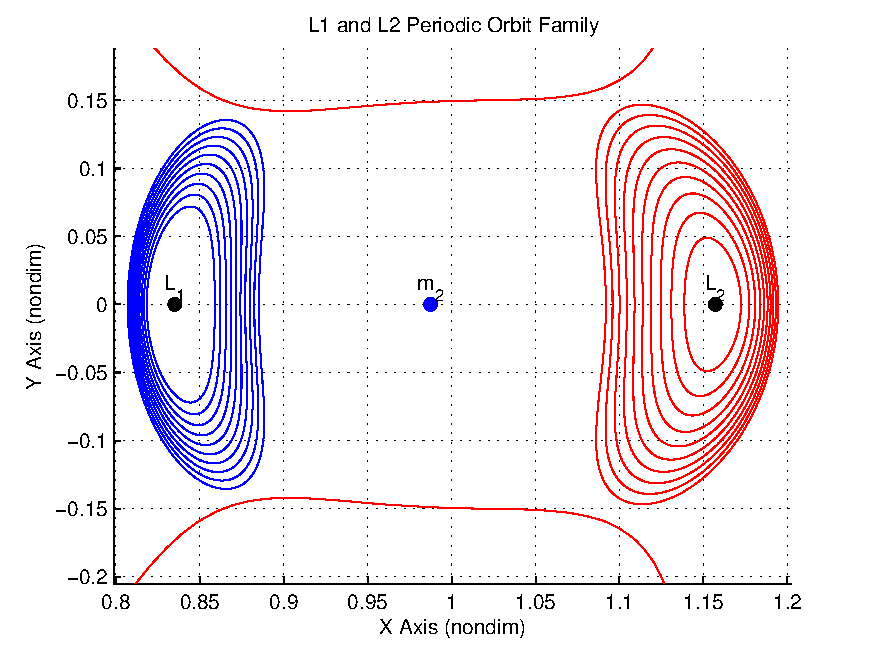
\includegraphics[width = 0.9\columnwidth]{L1L2_periodic_family}
			\caption*{Family of Periodic Orbits\label{fig:periodic_family}}
		\end{figure}
	\end{minipage}%end of right half of block
	% lots of pictures of the invariant manifolds
	\begin{figure}
        \centering
        \begin{subfigure}[b]{0.24\columnwidth}
                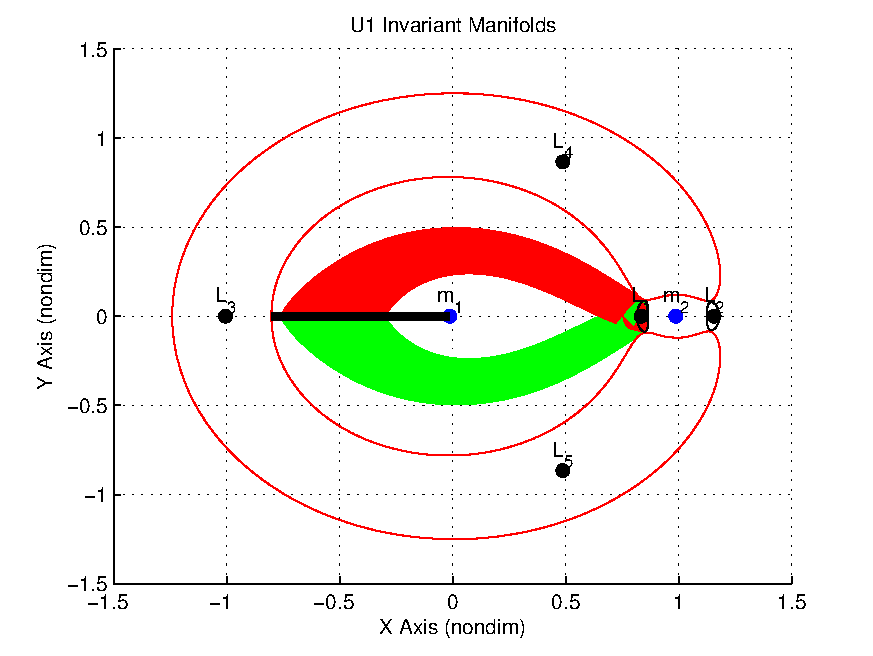
\includegraphics[width=\columnwidth]{U1_Manifolds}
                \caption*{U1 Manifolds}
                \label{fig:u1_manifolds}
        \end{subfigure}%
        ~%add desired spacing between images, e. g. ~, \quad, \qquad, \hfill etc.
          %(or a blank line to force the subfigure onto a new line)
        \begin{subfigure}[b]{0.24\columnwidth}
                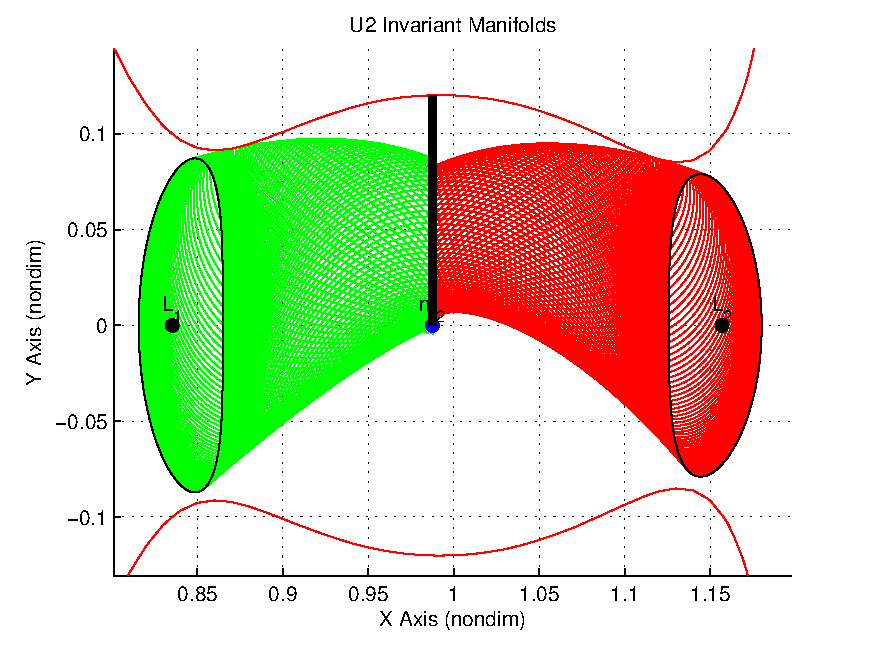
\includegraphics[width=\columnwidth]{U2_Manifolds}
                \caption*{U2 Manifolds}
                \label{fig:u2_manifolds}
        \end{subfigure}
        ~%
        \begin{subfigure}[b]{0.24\columnwidth}
                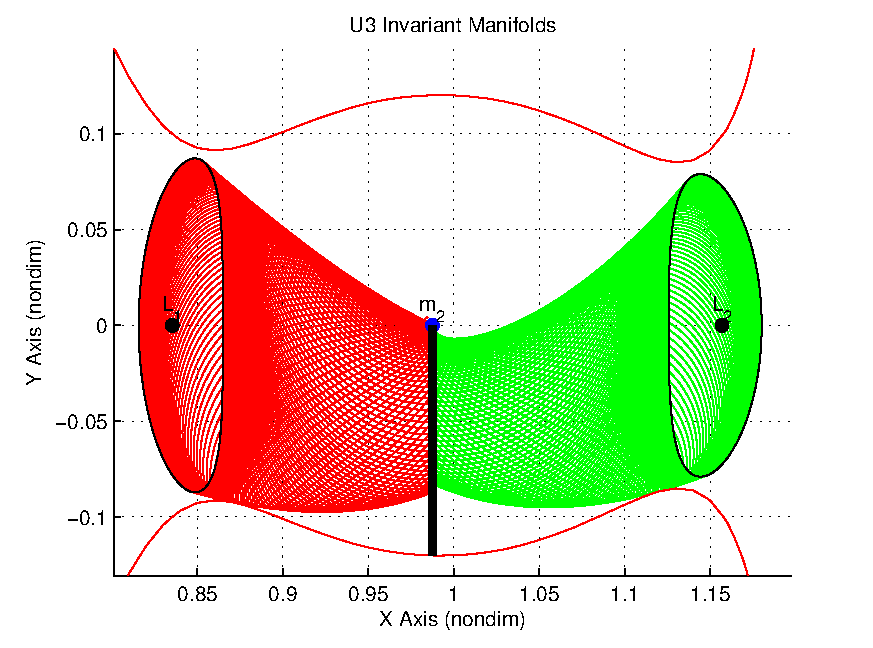
\includegraphics[width=\columnwidth]{U3_Manifolds}
                \caption*{U3 Manifolds}
                \label{fig:u3_manifolds}
        \end{subfigure}%
        ~%add desired spacing between images, e. g. ~, \quad, \qquad, \hfill etc.
          %(or a blank line to force the subfigure onto a new line)
        \begin{subfigure}[b]{0.24\columnwidth}
                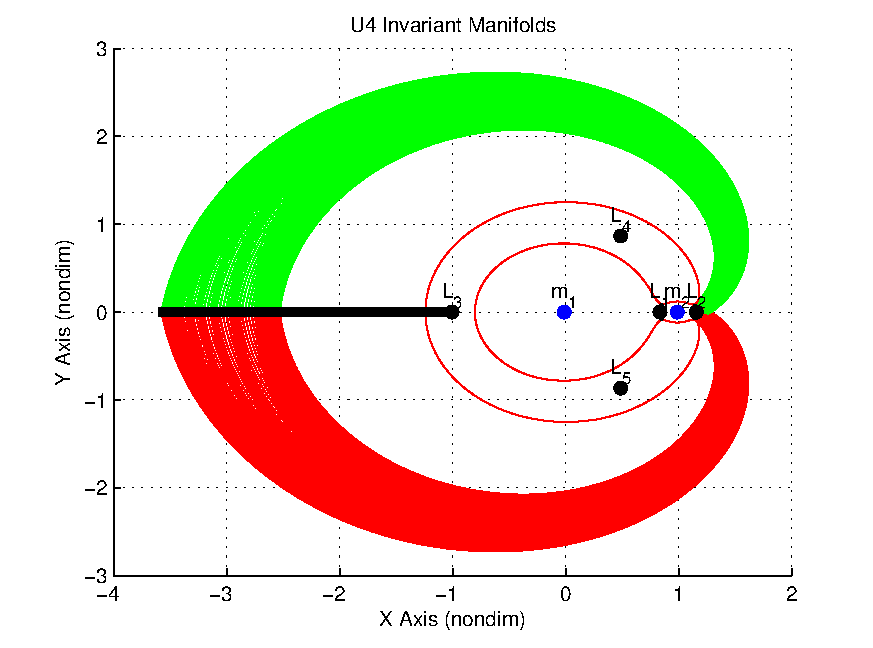
\includegraphics[width=\columnwidth]{U4_Manifolds}
                \caption*{U4 Manifolds}
                \label{fig:u4_manifolds}
        \end{subfigure}
		\label{fig:invariant_manifolds}
	\end{figure}
\end{block} % end of structure block

\begin{block}{IV. Optimal Control Formulation} % optimal control block
	\begin{itemize}
		\item \Emph{Poincar\'e Section}, or return map, is an essential tool in examining the behavior of periodic orbits
			\begin{itemize}
				\item Use of the Jacobi integral and intersection hyperplane reduces the problem dimensionality and allows for improved visualization
			\end{itemize}
		\begin{figure}
        	\centering
        	\begin{subfigure}[b]{0.24\columnwidth}
                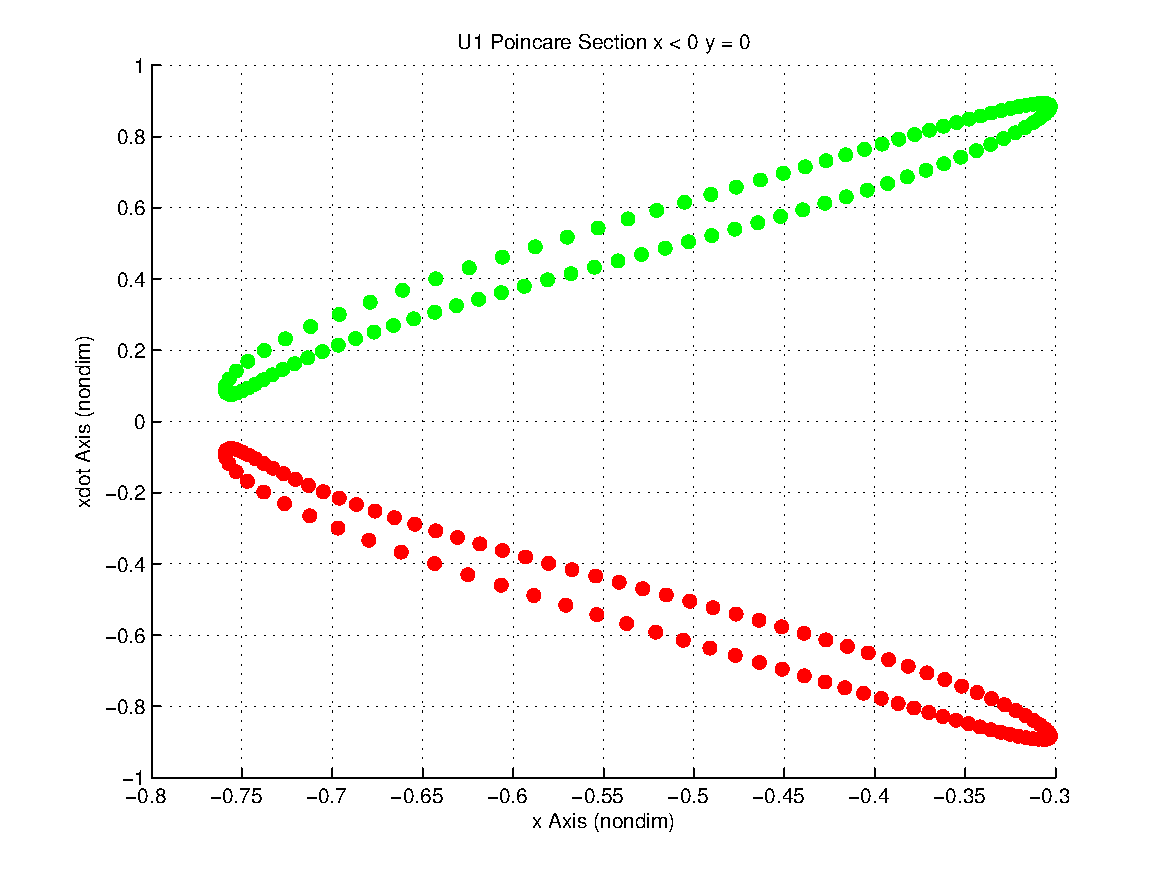
\includegraphics[width=\columnwidth]{U1_poincare}
                \caption*{U1 Poincar\'e}
                \label{fig:u1_poincare}
        	\end{subfigure}%
        	~%add desired spacing between images, e. g. ~, \quad, \qquad, \hfill etc.
          	%(or a blank line to force the subfigure onto a new line)
        	\begin{subfigure}[b]{0.24\columnwidth}
                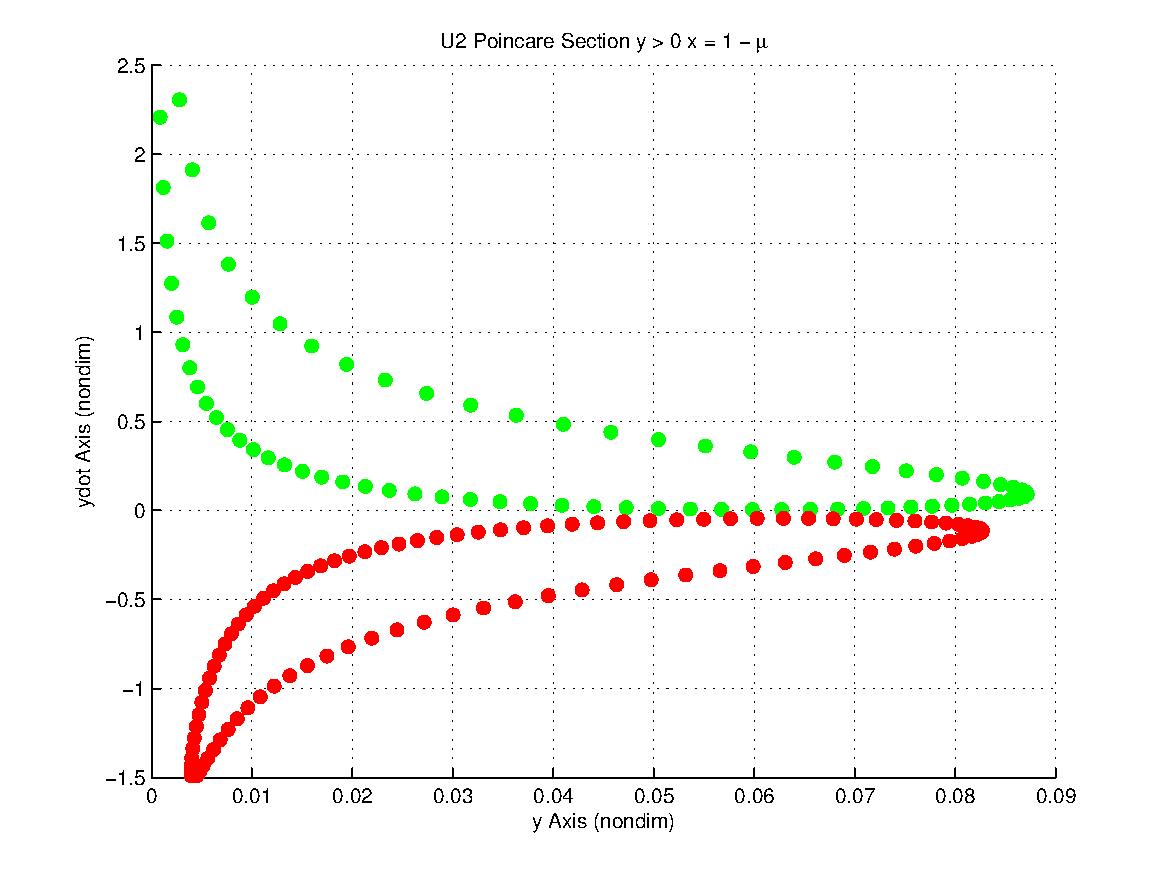
\includegraphics[width=\columnwidth]{U2_poincare}
                \caption*{U2 Poincar\'e}
                \label{fig:u2_manifolds}
        	\end{subfigure}%
        	~%
        	\begin{subfigure}[b]{0.24\columnwidth}
                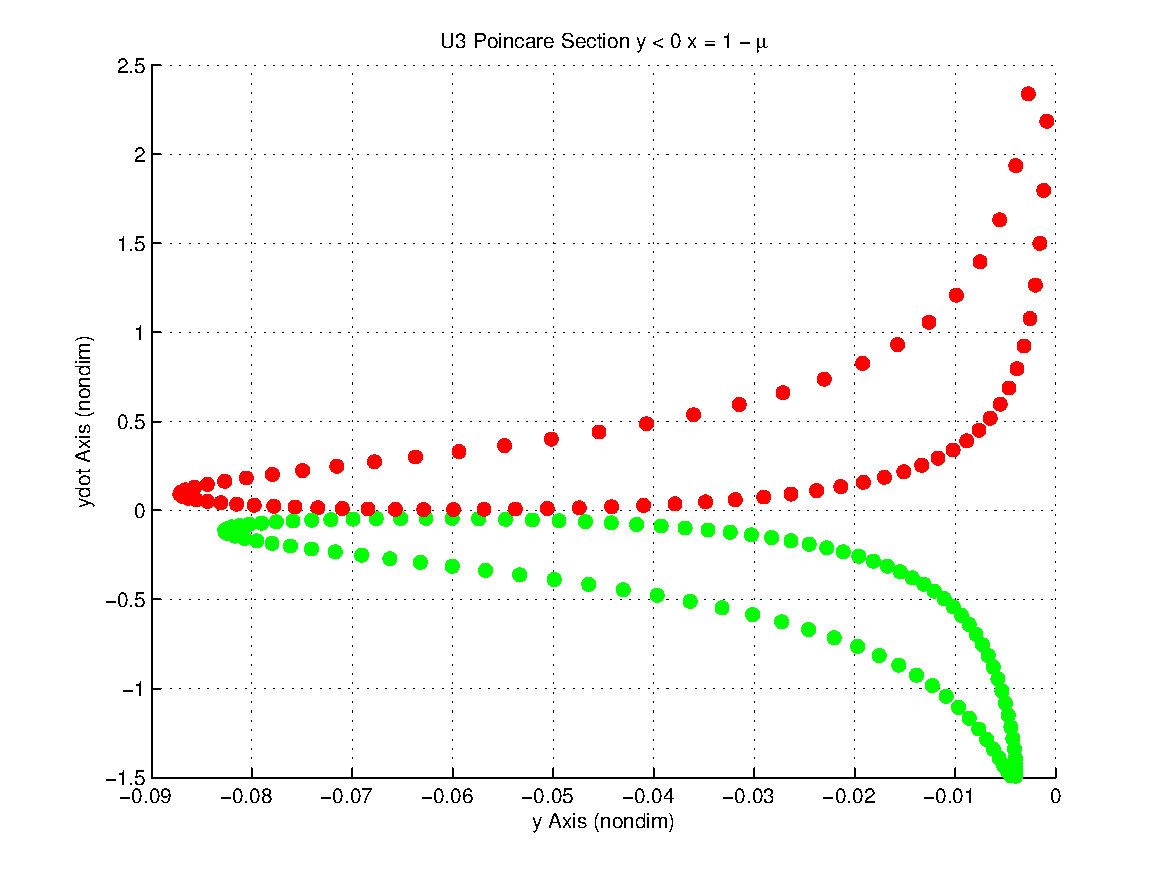
\includegraphics[width=\columnwidth]{U3_poincare}
                \caption*{U3 Poincar\'e}
                \label{fig:u3_poincare}
        	\end{subfigure}%
        	~%add desired spacing between images, e. g. ~, \quad, \qquad, \hfill etc.
          	%(or a blank line to force the subfigure onto a new line)
        	\begin{subfigure}[b]{0.24\columnwidth}
                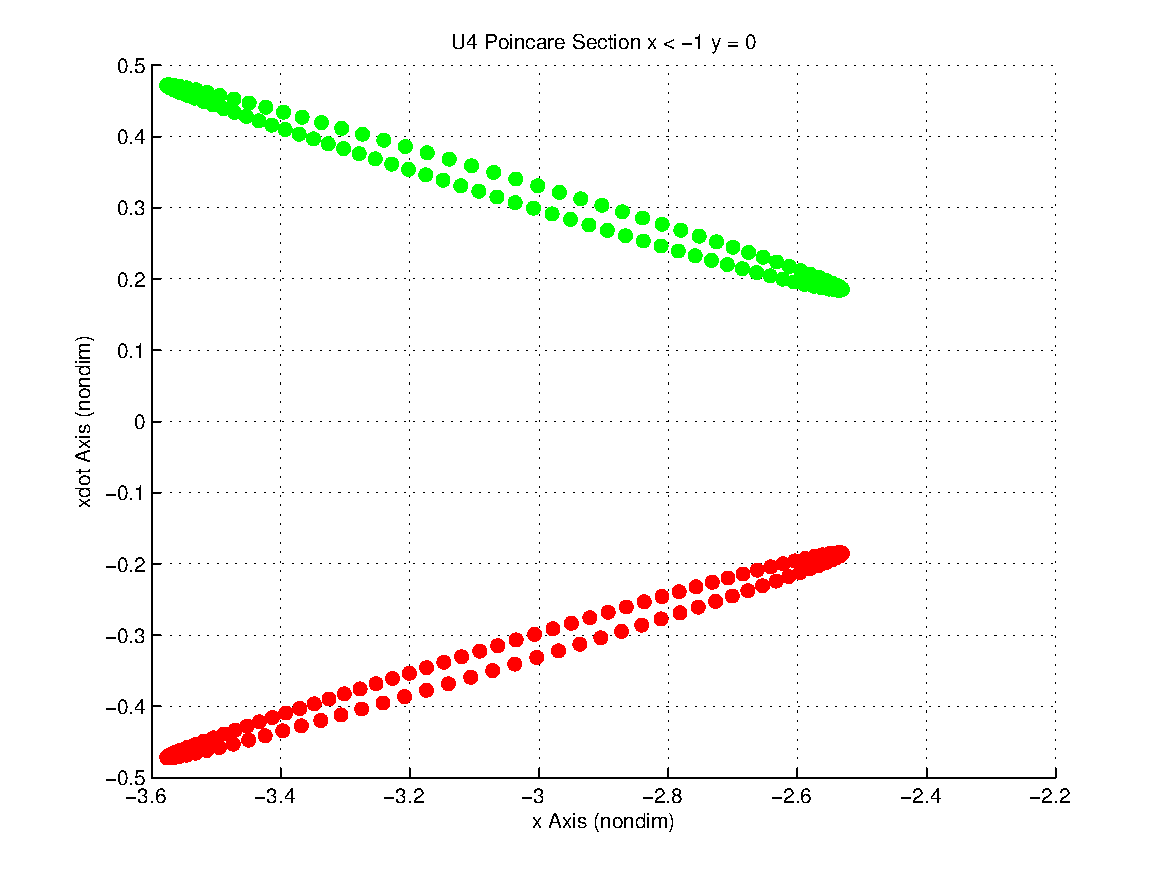
\includegraphics[width=\columnwidth]{U4_poincare}
                \caption*{U4 Poincar\'e}
                \label{fig:u4_poincare}
        	\end{subfigure}
			\label{fig:poincare_sections}
		\end{figure}
		\item \Emph{Optimal Control} techniques enables the design of control histories that allow transfers between regions of space
		\item Incorporating control magnitude constraints lets us approximate the reachable set of the spacecraft
			\begin{itemize}
				\item Calculus of variations leads to a two point boundary value problem with split boundary conditions
			\end{itemize}
			\begin{multicols}{2}
			\begin{equation*}
				\min J = -\frac{1}{2} \left( \bar{x}(t_f) - \bar{x}_{n}(t_f)\right)^T 
				\left[
					\begin{array}{cccc}
            		1 & 0& 0& 0 \\
            		 0& 0& 0& 0\\
            		 0 & 0 & 1 &0\\
            		 0 & 0& 0& 0
            	\end{array}
            	\right]
            	\left( \bar{x}(t_f) - \bar{x}_{n}(t_f)\right)
            	\label{eq:cost}
			\end{equation*}\break	
            \begin{align*}
            	 \frac{y(t_f) - L1_y}{x(t_f) - L1_x} - \tan{\alpha_d} &= 0\\ 
            	 \frac{\dot{x}(t_f) - \dot{x_n}(t_f) }{x(t_f) -x_n(t_f) } - \tan{\theta_d} &= 0\\
				 \bar{u}^T \bar{u} - u_{max}^2 &\leq 0
            	\label{eq:constraint}
            \end{align*}
			\end{multicols}
		\item Reachable set approximates state space that can be attained by spacecraft 
		\item Constraints ensure trajectories intersect the return map and maximize the attainable state
	\end{itemize}
\end{block} % end of optimal control block
\end{column}


%-----------------------------------------------------------------------------------------
% THIRD (RIGHT) COLUMN
%---------------------------------------------------------------------------------------
\begin{column}{\onecolwidth} % third column start

\begin{block}{V. Experimental Results} % results block
	\begin{itemize}
		\item Design control history that transfers spacecraft between periodic orbits about the Earth-Moon L1 Lagrange point
		\item An algorithm is developed that approximates the reachable state space on a chosen Poincar\'e section
		\begin{itemize}
			\item 2D Poincar\'e section allows straightforward visualization and decreases the problem complexity
			\item Variation of \( \theta_d \) generates the reachable set which approximates the states that can be achieved subject to the bounded control input
		\end{itemize}
		\begin{figure}
        	\centering
        	\begin{subfigure}[b]{0.46\columnwidth}
        		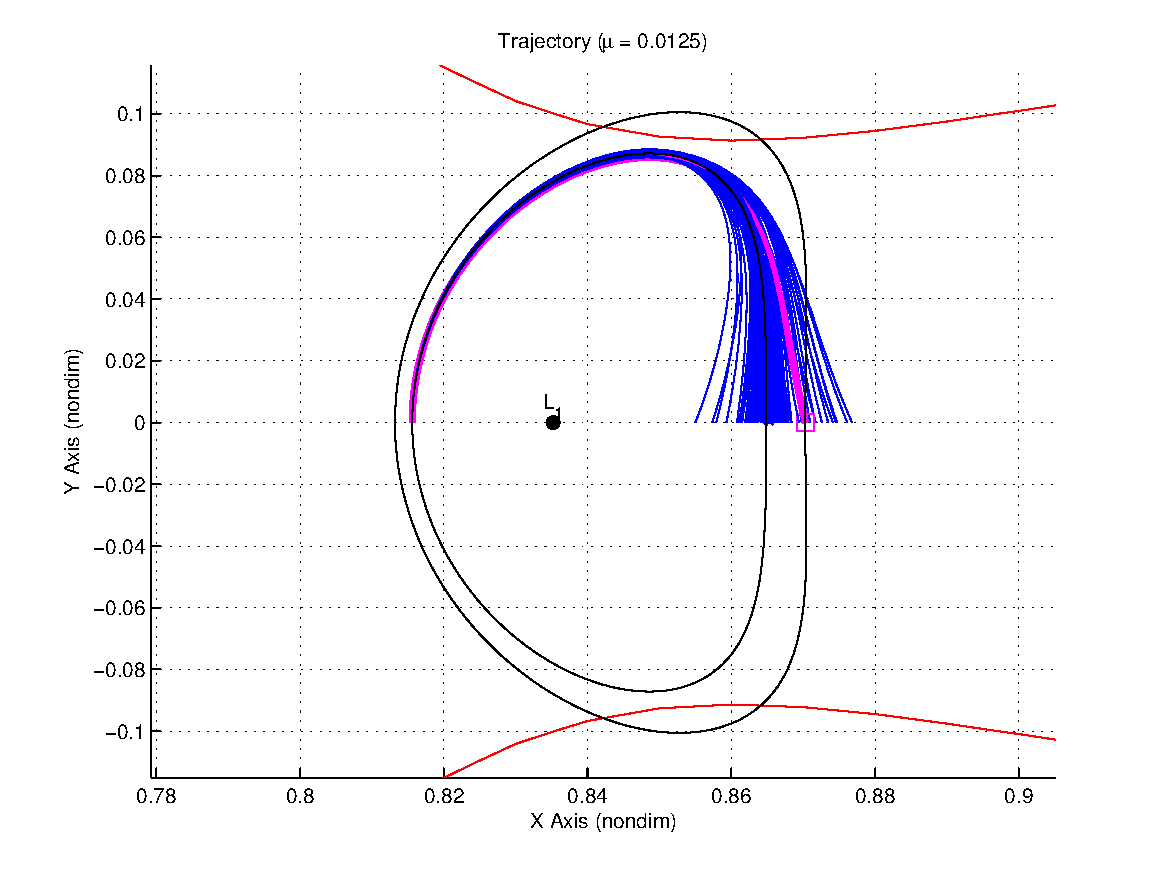
\includegraphics[width=\columnwidth]{north_reach_trajectory}
        		\caption*{Norther Reachable Trajectories}
        		\label{fig:north_trajectory}
        	\end{subfigure}%
			~%
			\begin{subfigure}[b]{0.46\columnwidth}
        		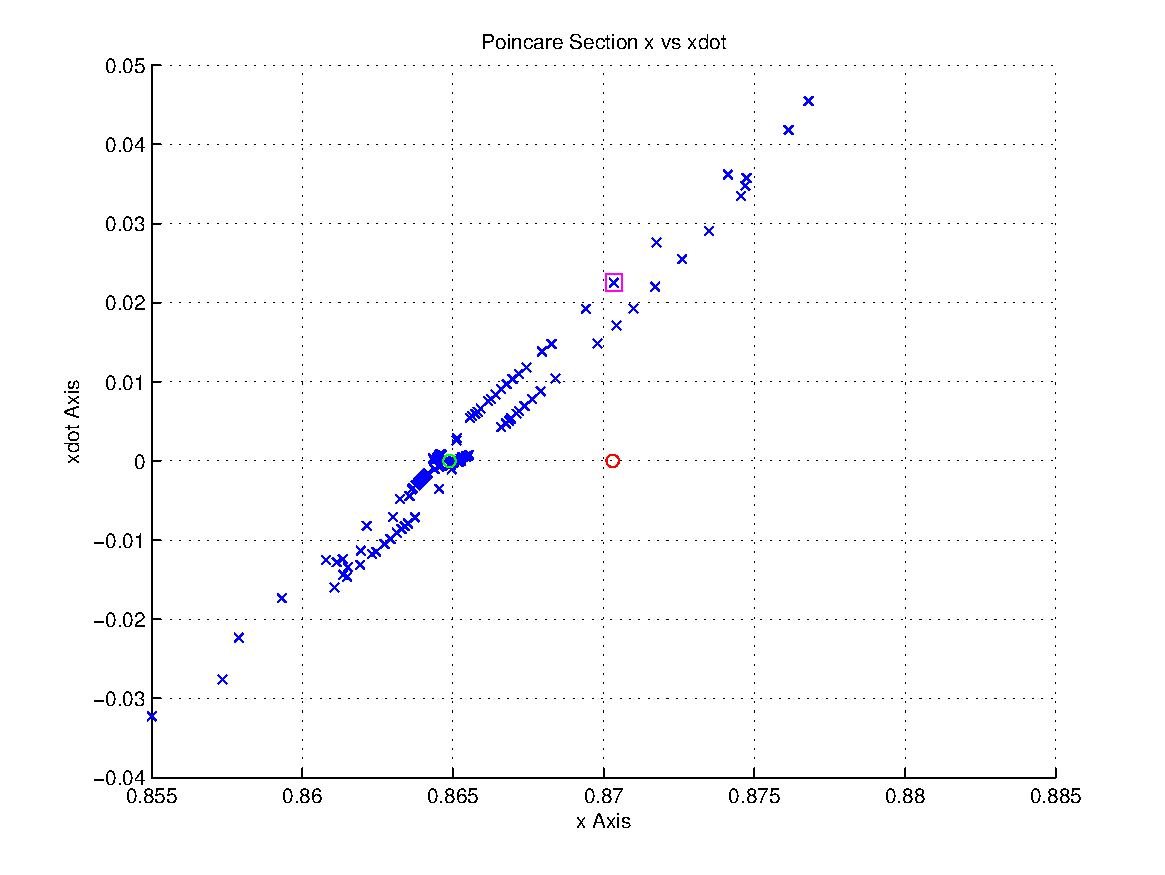
\includegraphics[width=\columnwidth]{north_reach_poincare}
        		\caption*{Northern Poncar\'e Reachable set }
        		\label{fig:north_poincare_reach}
        	\end{subfigure}
        \end{figure}
	\item Multiple iterations of the reachable set computation allows for transfer trajectory design 
		\begin{figure}
        	\centering
        	\begin{subfigure}[b]{0.46\columnwidth}
        		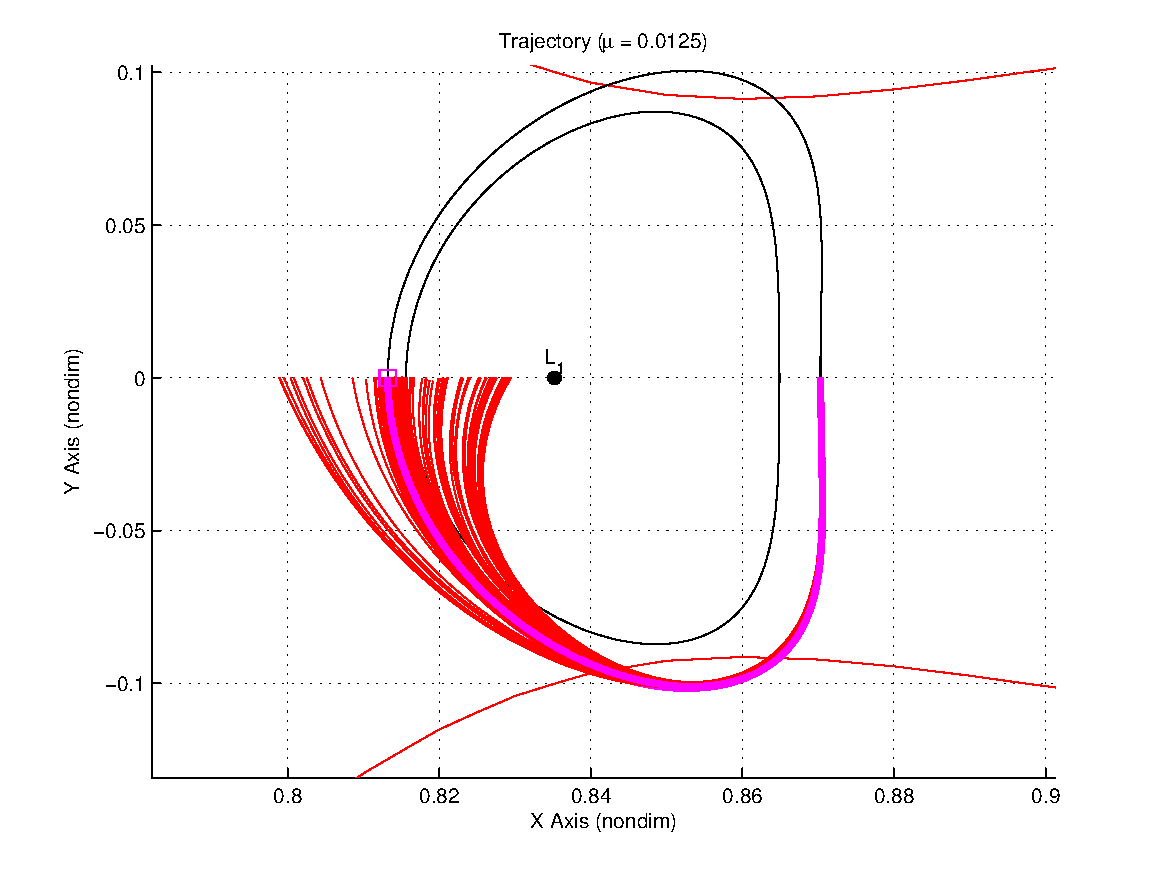
\includegraphics[width=\columnwidth]{south_reach_trajectory}
        		\caption*{Southern Reachable Trajectories}
        		\label{fig:south_trajectory}
        	\end{subfigure}%
			~%
			\begin{subfigure}[b]{0.46\columnwidth}
        		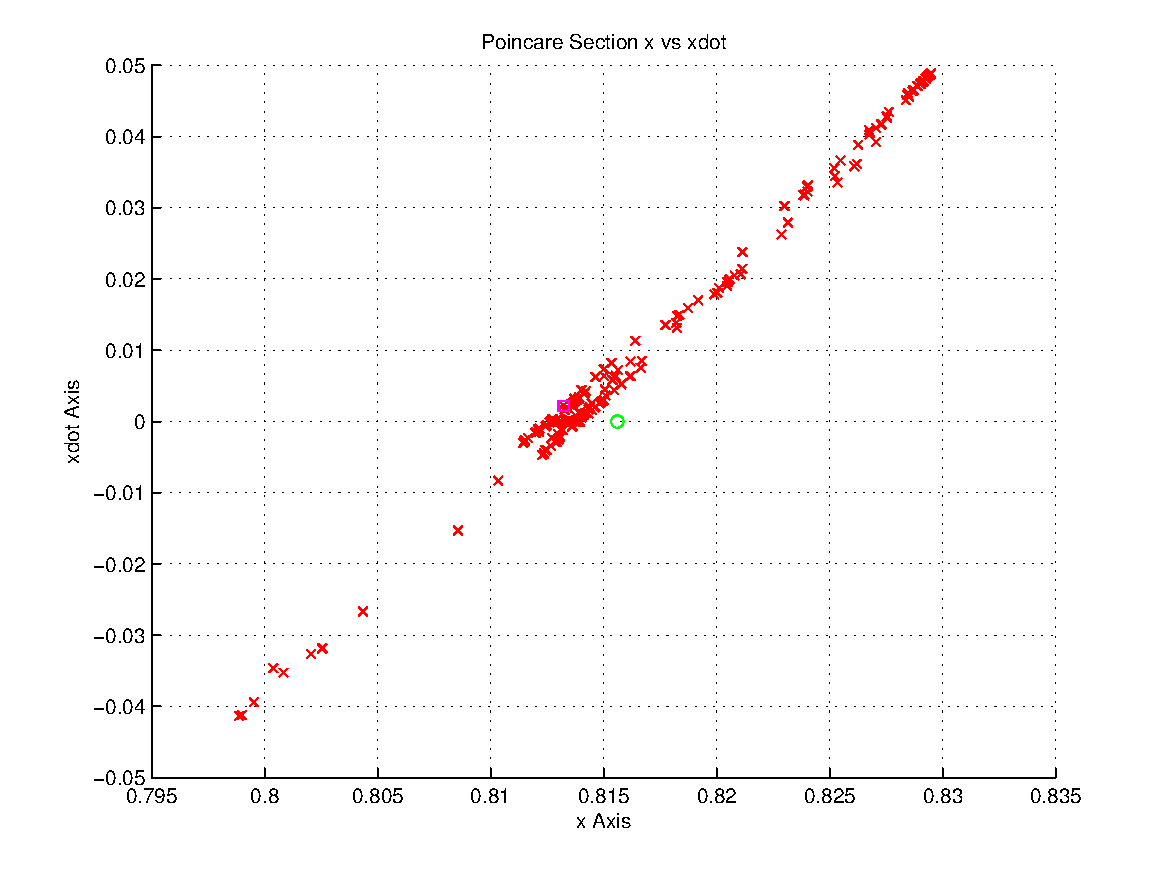
\includegraphics[width=\columnwidth]{south_reach_poincare}
        		\caption*{Southern Poncar\'e Reachable set }
        		\label{fig:south_poincare_reach}
        	\end{subfigure}
        \end{figure}	
    \item Poincar\'e section chosen such that periodic solutions will intersect the section twice per orbital period
    \item Projection of optimal trajectories onto the return map enables a decision making process in a lower dimensional space
\end{itemize}

\end{block} % end of results block

\begin{block}{VI. Conclusion} % conclusion
	\begin{itemize}
		\item Developed an optimal transfer design process which utilizes the concept of reachable sets on lower dimensional Poincar\'e maps
		\item Indirect optimal control formulation enables straightforward method of incorporating additional path and control constraints
		\item Current formulation is open loop and not robust to model uncertainties or disturbances. 
			\begin{itemize}
				\item Nonlinear Lyapunov theory is being pursued to develop a feedback control algorithm that offers verifiable stability properties
			\end{itemize}
		\item Planar assumption is a valid model for popular mission scenarios such as the Earth-Moon or Sun-Earth system
			\begin{itemize}
				\item Extension to the spatial problem is necessary for more exotic missions, such as multi-moon orbit missions of the outer planets
				\item Poincar\'e map representation would require extension from 2D to 4D 
				\item Innovative visualization techniques required to display higher dimensional state spaces
			\end{itemize}
	\end{itemize}
\end{block} % conclusion
\end{column}  % third column end

\end{columns} % end of all columns in poster
\end{frame} % end of enclosing frame
\end{document}